\documentclass{standalone}
\usepackage{tikz}

\begin{document}

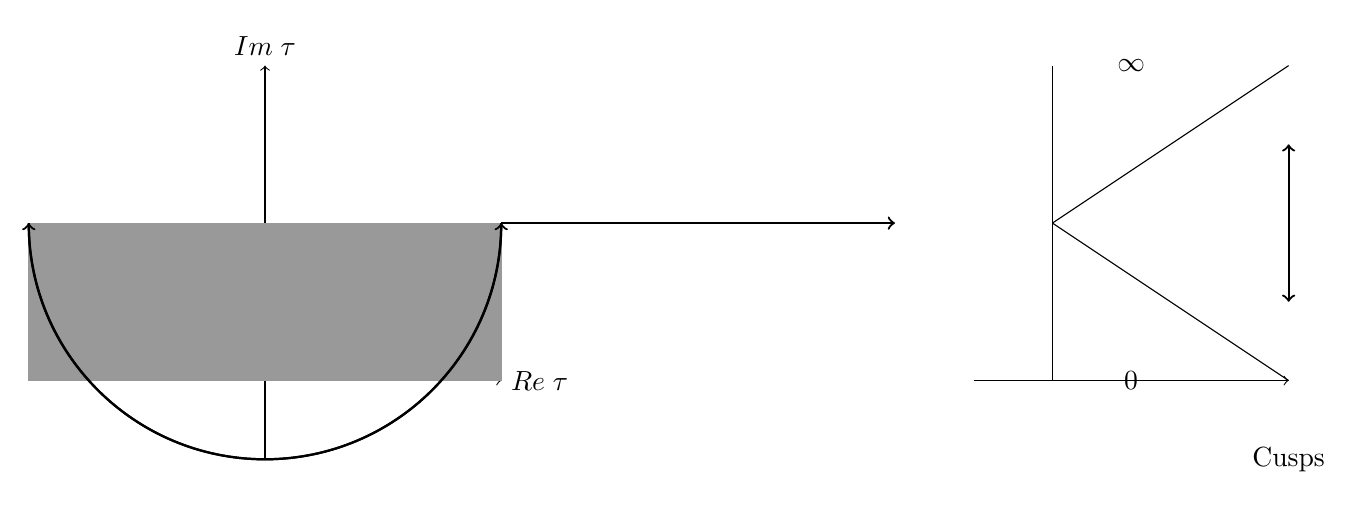
\begin{tikzpicture}[scale=2]

% Draw the complex plane
\draw[->] (-1.5,0) -- (1.5,0) node[right] {$Re \; \tau$};
\draw[->] (0,-0.5) -- (0,2) node[above] {$Im \; \tau$};

% Fill the region in the complex plane
\filldraw[gray!80] (-1.5,0) rectangle (1.5,1);

% Arrows indicating identification
\draw[->,thick] (-1.5,1) arc (180:360:1.5);
\draw[->,thick] (1.5,1) arc (0:-180:1.5);

% Arrow indicating the direction of the transformation
\draw[->,thick] (1.5,1) -- (4,1);

% Right side of the image
\draw[->] (4.5,0) -- (6.5,0) node[right] {};

% Draw the vertical line
\draw (5,0) -- (5,2);

% Label for the vertical line
\node at (5.5,2) {$\infty$};
\node at (5.5,0) {$0$};

% Draw the slanted lines
\draw (5,1) -- (6.5,2);
\draw (5,1) -- (6.5,0);

% Label for the cusps
\node at (6.5,-0.5) {Cusps};

% Arrows indicating the cusps
\draw[->,thick] (6.5,1) -- (6.5,0.5);
\draw[->,thick] (6.5,1) -- (6.5,1.5);

\end{tikzpicture}

\end{document}